
\chapter{Intégration sur un espace mesurable} % (fold)



\begin{tcolorbox}
Requirements : 
\begin{itemize}

    \item Topologie
    \item Suites et Séries 
    \item Familles sommables

    

\end{itemize}

Contents : 
\begin{itemize}

    \item Définitions
      \begin{enumerate}

          \item Tribu ($\sigma$-algèbre), tribu borélienne
          \item Mesure (positive, $\sigma$-finie)
          \item $\mu$-négligeable, presque partout (ou sûrment), $\mu$-complétée 
          \item Fonction mesurable, étagée
          \item Fonction intégrable
          \item Tribu image, mesure image
          \item $\mathscr{C}^k$-difféomorphisme

      \end{enumerate}

    \item Théorèmes, propositions, propriétés

    \begin{enumerate}
      \item Propriétés de fonction intégrable (linéarité, croissance, restriction, relation de Chasles)
 \item Théorème de convergence monotone
 \item Lemme de Fatou 
  \item Théorème de convergence dominée
  \item Tribu produit, mesure produit
  \item Théorème de Fubini-Tonelli, Fubini-Lebesgue (pas forcément savoir la démonstration)
  \item Changement de variable
  \item $\mathscr{C} ^{1}$-difféomorphisme

    \end{enumerate}

\end{itemize}
Last update : \textit{12 Novembre, 2023}, Shanghai
\end{tcolorbox}

\label{chap:Intégrabilité}

% chapter Intégrabilité (end)

\section{Espace mesurable} % (fold)
\label{sec:Espace mesurable}

\subsection{Topologie} % (fold)
\label{sub:Topologie}

% subsection Topologie (end)

Rappel : $\mathbb{R} \to \mathbb{R} ^{n} \to E \text{ de dimension finie} \to (E,d) \to E \text{ muni d'une topologie}$

\begin{Definition}[colbacktitle=red!75!black]{Topologie}{}
  Une \textbf{topologie} sur $E$ est un \underline{ensemble $\mathcal{TO}$ de parties de $E$} qui vérifie l'\underline{ensembles des ouverts de $E$}
  \begin{itemize}

      \item $\emptyset \in \mathcal{TO}$, $E \in \mathcal{TO}$ 
      \item Stabilité par réunion quelconque des ouverts : Si $(O_i) _{i \in I} \in \mathcal{TO} ^{I}$, alors $\bigcup _{i \in I} O_i \in \mathcal{TO}$ 
      \item Stabilité par intersection finie des ouverts : Si $n \in \mathbb{N} ^{*}$, $(O_1, \dots, O_n) \in \mathcal{TO} ^{n}$, $\bigcap _{k=1} ^{n} O_k \in \mathcal{TO}$.

  \end{itemize}
\end{Definition} 

\begin{note}{}{}
Ouf ! On ne va pas utiliser cette formalisation. Mais, on va souvent considérér $\mathcal{TO}$ \underline{les ouverts de $E$.}
\end{note}



\subsection{Tribu} % (fold)
\label{sub:Tribu}

% subsection Tribu (end)
\begin{Definition}[colbacktitle=red!75!black]{Tribu, $\sigma$-algèbre}{}
Une \textbf{tribu} ou $\sigma$-\textbf{algèbre} sur un ensemble \( \Omega \) est une collection \( \mathcal{T} \) de sous-ensembles de \( A \) qui possède les propriétés suivantes : \begin{itemize}

   \item Non vide : $\emptyset \in \mathcal{T}$

    \item Stabilité par \underline{passage au complémentaire} : $\forall A \in \mathcal{T}$, $A ^{c} \in \mathcal{T}$
    \item Stabilité par \underline{réunion dénombrable} : Soit $(A_n) _{n \in \mathbb{N}} \in \mathcal{T} ^{\mathbb{N}}$, alors $\bigcup _{n \in \mathbb{N}} A _n \in \mathcal{T}$

\end{itemize}

Les parties de $\mathcal{T}$ sont dites \textbf{parties mesurables}. On le note $(\Omega, \mathcal{T})$.
\end{Definition}

\begin{Definition}[colbacktitle=red!75!black]{Espace mesurable}{}
Un ensemble muni d'une \textbf{tribu} est dit \textbf{espace mesurable}. 
\end{Definition}



Mais on travaille la plupart du temps dans un espace vectoriel normé (ou un espace métrique). 

Pour faire le lien, on aimerait que les ouverts soient des parties mesurables. 

\begin{Definition}[colbacktitle=red!75!black]{Tribu borélienne}{}
  Si $(E,d)$ un espace métrique (donc on peut définir des boules), on appelle \textbf{tribu borélienne} {la plus petite tribu} contenant les \underline{ouverts} de $E$. On la note $\boxed{\mathcal{BO}(E)}$
\end{Definition}

\begin{myproof}{}{} Existence du \textbf{tribu borélienne} : 
  $\mathcal{F}= \{ \mathcal{T} \text{ tribu sur } E, \; \mathcal{T} \supset \mathcal{TO}\}$ (Rappel : $\mathcal{TO}$ est l'ensemble des ouverts de $E$)
  \begin{itemize}

      \item $\mathcal{F} \ne \emptyset$ car $\mathscr{P}(E) \in \mathcal{F}$ 
      \item $\mathcal{F}$ stable par intersection (très simple)

  \end{itemize}
  Donc, $\mathcal{BO}(E) = \bigcap _{\mathcal{T} \in \mathcal{F}} \mathcal{T}$ est la plus petite tribu contenant $\mathcal{TO}$
\end{myproof}

\begin{Prop}{Tribu borélienne dans $\mathbb{R}$}{}
Dans $\mathbb{R}$, les ouverts sont réunions \textbf{dénombrables} d'intervalles ouverts. (Vois cours topologie)

Donc,
\begin{itemize}

    \item Tribu borélienne
\begin{center}
  $\mathcal{BO}(\mathbb{R})$ = Plus petit tribu contenant tous les $]a,b[$
\end{center}

\item Tous les intervalles de $\mathbb{R}$ sont dans $\mathcal{BO}(\mathbb{R})$.

\end{itemize}
\end{Prop}

\begin{myproof}{}{}
Une tribu $\mathcal{T}$ est stable par réunion finie ou dénombrable, donc aussi stable par intersection finie ou dénombrable : soit $(B_0, \dots, B_n ) \in \mathcal{T} ^{n+1}$, on construisons $A_0 = B_0, \dots, A_n = B_n, \; \forall k >n, A _{k} = \emptyset \in \mathcal{T}$ (Formule de Moivre) 
\begin{equation}
  \left( \bigcup _{n \in \mathbb{N}} A_n \right) ^{c} = \bigcap_{n \in \mathbb{N}}^{} ( A_n ^{c})
\end{equation}
On peut construire tout intervalle sur \(\mathbb{R}\) à partir des ensembles ouverts, des complémentaires, et des intersections dénombrables : 
\begin{equation}
  [a,b] = \left( ]- \infty, a[ \cup ]b, + \infty[ \right) ^{c} \in \mathcal{T}
\end{equation}
\end{myproof}


\begin{Example}{}{}
  Dans $\mathbb{R} ^{n}$, $\mathcal{BO}(\mathbb{R} ^{n})$ = plus petite tribu contenant $\prod _{k=1} ^{n}]a_k,b_k[$
\end{Example}









\begin{Prop}{Tribu produit}{}
Soient $(\Omega_1, \mathcal{T}_1)$ et $(\Omega_2, \mathcal{T}_2)$ deux \textbf{espaces mesurables}, on appelle \textbf{tribu produit} sur $\Omega_1 \times \Omega_2$ et on note $\mathcal{T}_1 \otimes \mathcal{T}_2$ \underline{la plus petite tribu} contenant $A_1 \times A_2$ où $A_1 \in \mathcal{T}_1$ et $A_2 \in \mathcal{T}_2$.
\end{Prop}

\subsection{Mesure} % (fold)
\label{sub:Mesure}

% subsection Mesure (end)
\begin{Definition}[colbacktitle=red!75!black]{Mesure (positive)}{}
  Soit $(\Omega, \mathcal{T})$  un espace mesurable, on appelle \textbf{mesure (positive)} sur $\Omega$, toute \underline{application} $\mu : \mathcal{T} \to \mathbb{R}_+ \cup \{ + \infty\}$ et qui vérifie :
  \begin{itemize}

      \item $\mu(\emptyset) = 0$ 
      \item \underline{$\sigma$-additivité (dénombrable)} : $\forall (A_n) _{n \in \mathbb{N}} \in \mathcal{T} ^{\mathbb{N}}$, disjointes 2 à 2, $\mu(A_n) _{n \in \mathbb{N}}$ nécessairement sommable.
        \begin{equation}
          \forall (A_n) _{n \in \mathbb{N}} \in \mathcal{T} ^{\mathbb{N}}, \; \left[\forall (i,j) \in \mathbb{N} ^{2}, [i \ne j] \implies [A_i \cap A_j = \emptyset]\right] \implies \boxed{\mu \left( \bigcup _{n \in \mathbb{N}} A_n \right) = \sum_{n \in \mathbb{N}}^{} \mu(A_n)}
        \end{equation}

  \end{itemize}

  $(\Omega, \mathcal{T}, \mu)$ s'appelle \textbf{espace mesuré}.
\end{Definition}

\begin{Theorem}{Mesure de Lebesgne ($\mathbb{R}$)}{}
 Dans $\mathbb{R}$, il \underline{existe} une \underline{unique} mesure (dite \textbf{mesure de Lebesgne} et notée $\lambda$) sur $\mathcal{BO}(\mathbb{R})$ qui vérifie
\begin{equation}
  \forall (a,b) \in \mathbb{R} ^{2}, \; [a<b] \implies [\lambda(]a,b[) = b-a]
\end{equation}
\end{Theorem}

\begin{myproof}{}{}
Admis.
\end{myproof}
\begin{Theorem}{Mesure de Lebesgne ($\mathbb{R} ^{n}$)}{}
 Dans $\mathbb{R}$, il \underline{existe} une \underline{unique} mesure (dite \textbf{mesure de Lebesgne} et notée $\lambda$) sur $\mathcal{BO}(\mathbb{R } ^{n})$ qui vérifie

\begin{equation}
  \forall k \in [\!1, n]\!], [a_k \le b_k] \implies \lambda \left( \prod_{k=1}^{n}]a_k, b_k[ \right) = \prod_{k=1}^{n} (b_k - a_k)
\end{equation}
\end{Theorem}

\begin{Example}{Mesure de comptage sur les parties}{}
\begin{equation}
  \forall A \subset \Omega, \; \mu(A) = \begin{cases}
  + \infty \text{ si } A \text{ est infini} \\ 
  \mathrm{card}(A) \text{ sinon }
  \end{cases}
\end{equation}
\end{Example}

\begin{Example}{Mesure de comptage des entiers sur les parties de $\mathbb{R}$}{}
\begin{equation}
  \forall A \subset \Omega, \; \mu(A) = \begin{cases}
  + \infty \text{ si } A \in \mathbb{N} \text{ est infini} \\ 
  \mathrm{card}(A \cap \mathbb{N}) \text{ sinon }
  \end{cases}
\end{equation}
\end{Example}


\begin{Prop}{Propriétés d'un espace mesuré}{}
Soit $(\Omega, \mathcal{T},\mu)$ un espace mesuré (resp. $(\Omega, \mathcal{T}, \mathbb{P})$ un espace probabilisé) : 

\begin{note}{}{}
Remplacer $\mu$ par $\mathbb{P}$ et on retrouve les résultats dans le cours de probabilité.
\end{note}


\begin{itemize}

    \item Croissance : 
      \begin{equation}
        \forall (A, B) \in \mathcal{T} ^{2}, \; [A \subset B] \implies [\mu(A) \le \mu(B)]
      \end{equation}

    \item Réunion + Intersection : 
      \begin{equation}
        \forall (A, B) \in \mathcal{T} ^{2}, \; \mu(A) + \mu(B) = \mu(A \cap B) + \mu (A \cup B)
      \end{equation} 

    \item Limite croissante : 

      \begin{equation}
        \forall (A_n) _{n \in \mathbb{N}} \in \mathcal{T} ^{\mathbb{N}}, \; [\forall n \in \mathbb{N}, A_n \subset A _{n+1}] \implies \left[ \mu \left( \bigcup _{n\in \mathbb{N}} A_n \right)\right] = \lim _{n \to + \infty} \mu (A_n)
      \end{equation}

    \item Limite décroissante 

      \begin{equation}
        \forall (A_n) _{n \in \mathbb{N}} \in \mathcal{T} ^{\mathbb{N}}, \; \mu(A_0) \ne + \infty, \; [\forall n \in \mathbb{N}, A_n \supset A _{n+1}] \implies \left[ \mu \left( \bigcap _{n\in \mathbb{N}} A_n \right)\right] = \lim _{n \to + \infty} \mu (A_n)
      \end{equation}



      \begin{tcolorbox}
        On note les deux limites : 
        \begin{equation}
          \lim _{n \to + \infty} \uparrow \mu (A_n), \quad 
          \lim _{n \to + \infty} \downarrow \mu (A_n)
          \label{eq: 2.11}
        \end{equation}
      \end{tcolorbox}
    \item Sous $\sigma$-addivité : 
      \begin{equation}
        \forall (A_n) _{n \in \mathbb{N}} \in \mathcal{T} ^{\mathbb{N}}, \; \mu \left( \bigcup _{n \in \mathbb{N}} A_n\right) \le \sum_{k \in \mathbb{N}}^{} \mu(A_k)
      \end{equation}

\end{itemize}
\end{Prop}

\begin{myproof}{}{}
Soit $(A,B) \in \mathcal{T} ^{2}$, 
\begin{itemize}

    \item $A \subset B$ donc $B = A \cup (B \backslash A)$. De plus $B \backslash A = B \cap A ^{c}$, donc 
      \begin{equation}
        \mu(B) = \mu(A) + \mu(B \backslash A) \ge \mu(A)
      \end{equation}

    \item Si $\mu(A \cup B) = + \infty$ alors $\mu(A) = + \infty$ ou $\mu(B) = +\infty$. Puisque, sinon, 
      \begin{equation}
        A \cup B = A \cup (B \backslash A) \implies \mu (A \cup B) = \mu(A) + \mu(B \backslash A)\le \mu(A) + \mu(B)
      \end{equation}

      Si $\mu(A \cup B) < + \infty$, considérer $B = (A \cap B) \cup (B \backslash A)$

    \item Construisons $B_n = A _{n } \backslash A _{n -1}$, $B_0 = A_0$. 
      \begin{itemize}

          \item 
            \begin{equation}
              \bigcup _{n \in \mathbb{N}} A_n = \bigcup _{n \in \mathbb{N}} B_n
            \end{equation}

          \item 
            \begin{equation}
              \mu \left( \bigcup _{n \in \mathbb{N}} A_n \right) = \sum_{n\in \mathbb{N}}^{} \mu(B_n) = \mu(B_0) = \sum_{n \in \mathbb{N}}^{}  \left( \mu (A_n) - \mu (A _{n-1})\right)  \underset{n \to + \infty}{\longrightarrow}  \mu(A_n)
            \end{equation}


      \end{itemize}

    \item $A_0 \backslash \bigcap _{n \in \mathbb{N}} A_n$, appliquer la limite croissante.
    \item Construisons $B_0 = A_0$, $B _n = A_n \backslash \left( \bigcup _{k=0} ^{n-1} A_k \right)$
\end{itemize}

\end{myproof}

\subsection{Négligeable, Presque partout, presque sûrement} % (fold)

% subsection Presque partout, presque sûrement (end)

\begin{Definition}[colbacktitle=red!75!black]{$\mu$-négligeable}{}
Soit $(\Omega, \mathcal{T}, \mu)$ un ensemble mesuré, soit $A \subset \Omega$, on dit que $A$ est $\mu$-\textbf{négligeable} si :

\begin{equation}
  \exists T \in \mathcal{T}, \; A \subset T, \text{ et } \mu(T) = 0
\end{equation}
\end{Definition}


\begin{Prop}{}{}
Dans $\mathbb{R}$ ($\mathbb{R} ^{n}$), tout ensemble dénombrable est de mesure nulle. 
\end{Prop}


\begin{Example}{Mesure nulle}{}
\begin{itemize}

    \item Ensemble dénombrable : $\lambda ( \mathbb{Q}) = 0$ en effet, $\mathbb{Q} = \bigcup _{q \in \mathbb{Q}} \{q\}$ donc $\lambda(\mathbb{Q}) = \sum_{q \in \mathbb{Q}}^{}\lambda(\{q\}) = q-q =0$
    \item Ensemble non dénombrable (Ensemble de Cantor) : 
      \begin{equation}
        K = \left\{ x \in [0,1], \; \exists (\varepsilon_k) _{k \in \mathbb{N}} \in \{0, 2 \} ^{\mathbb{N}}, \; x = \sum_{k=0}^{ + \infty} \frac{\varepsilon_k}{3 ^{k+1}} \right\}
      \end{equation}
      est $\lambda$-négligeable mais pas dénombrable.

      \begin{figure}[H] %h:当前位置, t:顶部, b:底部, p:浮动页
        \centering
        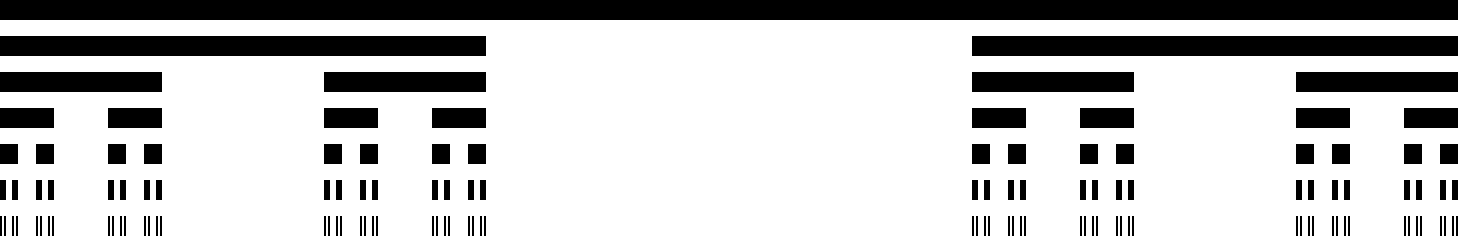
\includegraphics[width=0.8\textwidth]{./assets/Ensemble de Cantor.svg.png}
        \caption{Ensemble de Cantor}
        \label{fig:Ensemble de Cantor}
      \end{figure}

      
\end{itemize}
\end{Example}

\begin{myproof}{}{}
L'ensemble de Cantor est créé en enlevant répétitivement le tiers moyen d'un intervalle. Chaque point dans l'ensemble de Cantor peut être représenté de manière unique par une série infinie de 0 et de 2, cette représentation est similaire à une représentation binaire, donc bijection à $\mathbb{R}$. Donc, elle n'est pas dénombrable.
\end{myproof}








\begin{Definition}[colbacktitle=red!75!black]{$\mu$-presque partout, $\mu$-presque sûrement}{}
\begin{itemize}

  \item Soit $(\Omega, \mathcal{T}, \mu)$ un espace \underline{mesuré} et $P$ une propriété définie sur $\Omega$. On dit que $P$ est \textbf{vraie ($\mu$)-presque partout} si 
    \begin{center}
      $\{\omega \in \Omega, \; P(\omega) \text{ est fausse}\}$ est $\mu$-négligeable
    \end{center}
  \item Soit $(\Omega, \mathcal{T}, \mathbb{P})$ un espace \underline{probabilisé} et $P$ une propriété définie sur $\Omega$. On dit que $P$ est \textbf{vraie ($\mu$)-presque sûrement} si 
    \begin{center}
      $\{\omega \in \Omega, \; P(\omega) \text{ est fausse}\}$ est $\mu$-négligeable
    \end{center}

\end{itemize}

On les note resp. $P$ vraie $(\mu)$-p.p. et $P$ vraie ($\mathbb{P}$)-p.s.
\end{Definition}

\begin{Example}{}{}
Soit $(\Omega, \mathcal{T}, \mathbb{P})$. Soit $X$ une variable aléatoire réelle suivant une loi uniforme $\mathcal{U}(0,1)$, alors : $X \in [0,1]$ p.s.
\end{Example}

\subsection{Partie négligeable, complétée} % (fold)
\label{sub:}

% subsection  (end)
\begin{Definition}[colbacktitle=red!75!black]{Partie $\mu$-négligeable}{}

  Soit $(\Omega, \mathcal{T}, \mu)$ un espace mesuré. Une partie $A$ de $\Omega$ est dite $\mu$-\textbf{négligeable} s'il existe 
  \begin{equation}
    T \in \mathcal{T}, \; A \subset T, \; \mu(T) = 0
  \end{equation}
\end{Definition}


\begin{Definition}[colbacktitle=red!75!black]{$\mu$-complétée}{}
Soit $(\Omega, \mathcal{T}, \mu)$ un espace mesuré, on pose 
\begin{equation}
  \mathcal{N} = \{A \subset \Omega , A \;\mu-\text{négligeable}\}
\end{equation}



On appelle \textbf{tribu $\mu$-complétée} de $\mathcal{T}$ la tribu définie par 
\begin{equation}
  \boxed{\mathcal{T} ^{*} = \{ T \cup N,\; T \in \mathcal{T}, \; N \in \mathcal{N}\}}
\end{equation}

Le mesure $\mu$ se prolonge à $\mathcal{T} ^{*}$ par $\forall A \in \mathcal{T} ^{*}, \; \mu ^{*}(T \cup N) = \mu(T)$.
\end{Definition}




\newpage

\section{Intégrale de Lebesgne} % (fold)

\subsection{Fonction mesurable} % (fold)
\label{sub:Fonction mesurable}

\begin{tcolorbox}
    On voulait créer une intégrale sur des fonctions $f: \Omega \to \mathbb{R}$ où $(\Omega, \mathcal{T},\mu)$ un espace mesuré. Quelle propriété faut-il à $f$ pour pouvoir définir son intégrale ?
\end{tcolorbox}

\begin{Definition}[colbacktitle=red!75!black]{Fonction mesurable}{}
Soit $(\Omega, \mathcal{T})$, $(\Omega', \mathcal{T}')$ deux espaces mesurables. 
$f: \Omega \to \Omega'$ est dite \textbf{mesurable} si 
\begin{equation}
  \forall T' \in \mathcal{T} ', \; f ^{-1} (T') \in \mathcal{T}
\end{equation}
\end{Definition}

% subsection Fonction mesurable (end)
Remarque : 
\begin{itemize}

    \item Lorsque $(\Omega', \mathcal{T}')= (\mathbb{R}, \mathcal{BO}(\mathbb{R}))$, si $f$ est \textbf{mesurable}, $f ^{-1}(]a,b[) \in \mathcal{T}$. (Rappel : La plus petite tribu contenant les ouverts de $\mathbb{R}$)
    \item De plus, si $\mathcal{T}$ est la tribu borélienne de $(\Omega, d)$ alors, $f$ continue sur $\Omega$ donc $f$ mesurable sur $\Omega$.

\end{itemize}
\begin{Definition}[colbacktitle=red!75!black]{Fonction mesurable (2eme édition)}{}

  
Soit $(\Omega, \mathcal{T})$ et $f : \Omega \to [-\infty, + \infty]$, on dit que $f$ est \textbf{mesurable} si 
\begin{equation}
  \forall A \in \mathcal{BO}(\mathbb{R}),\; f ^{-1}(A) \in \mathcal{T}
\end{equation}
\end{Definition}

\subsection{Fonction étagée} % (fold)
\label{sub:Fonction étagée}

\begin{note}{}{}
  Rappel : Notation semblable à \textbf{Fonctions en escalier}, découplage de $[a,b]$
\end{note}
% subsection Fonction étagée (end)
\begin{Definition}[colbacktitle=red!75!black]{Fonctions étagées}{}

Soit $(\Omega, \mathcal{T})$ et $f : \Omega \to [-\infty, + \infty]$ à valeurs réels, on dit que $f$ est \textbf{étagée} si 
\begin{itemize}

    \item $f$ est \textbf{mesurable}
    \item et $\mathrm{card}(f(\Omega))$ est fini

\end{itemize}
\end{Definition}

\begin{Prop}{}{}
  Une \textbf{fonction en escalier} sur $[a,b]$ est étagée.
\end{Prop}

\begin{myproof}{}{}
\begin{itemize}

    \item Continue par morceaux donc mesurable 
    \item Prenant un nombre fini de valeurs

\end{itemize}
\end{myproof}

\begin{Example}{Fonction étagée}{}
  Fonction étagée $\xi_ \mathbb{Q} : \mathbb{R} \to \mathbb{R}$ :
\begin{equation}
  \xi _{\mathbb{Q}} : x \mapsto \mathbb{1} _{\mathbb{Q}}
\end{equation}
\end{Example}

\begin{Prop}{}{}
Soit $(\Omega, \mathcal{T}, \mu)$, toute focntion positive et mesurable est \underline{limite croissante} d'une suite de fonctions \underline{étagées positives}.
\end{Prop}

\subsection{Intégrale} % (fold)
\label{sub:Intégrale}

% subsection Intégrale (end)
\begin{Definition}[colbacktitle=red!75!black]{Intégrale}{}
\begin{enumerate}

    \item Soit $f$ une fonction \underline{étagée}, positive, définie sur $\Omega$, on pose 
      \begin{equation}
        \int_{\Omega}^{} f \mathrm{d} \mu = \sum_{\alpha \in f(\Omega)}^{} \alpha \mu (f ^{-1} ( \{\alpha\})) \in [0, + \infty]
      \end{equation}

    \item Soit $f$ une fonction \underline{positive}, mesurable définie sur $\Omega$, donc 
      \begin{equation}
        \int_{\Omega}^{} f \mathrm{d} \mu = \underset{g \in \Sigma_f}{\sup} \left( \int_{\Omega}^{} g \mathrm{d} \mu\right) \in [0, + \infty]
      \end{equation}
      où $\Sigma _f = \{g : \Omega \to \mathbb{R}_ + , \; g \text{ étagée et } g \le f \}$. 

      Notation : Si $\alpha = 0$ et $\mu(f ^{-1}(\{0\})) = + \infty$, alors $\alpha \mu( f ^{-1} (\{\alpha\})) = 0$

\end{enumerate}
\end{Definition}


\section{Intégrabilité} % (fold)

\subsection{Existence d'intégrale de Riemann} % (fold)
\label{sub:Existence d'intégrale de Riemann}

Le problème est que on souhaite de montrer $f$ est intégrable sur $I$, un intervalle donné, supposons $]a,b[$ ou $]a,b]$ ou etc.
\begin{itemize}

    \item Continuité sur un intervalle fermé, ou après un prolongement de la fonction 
    \item On peut trouver $c \in [a,b]$ tels que les deux limites existent : 
\begin{equation}
  \underset{\alpha \to a ^{+}}{\lim} \int_{\alpha}^{c} f(x) \mathrm{d}x , \quad \underset{\beta \to b ^{-}}{\lim} \int_{c}^{\beta} f(x) \mathrm{d}x
\end{equation}
    \item Comparaison asymptotique avec une intégrale de Riemann convergente

\end{itemize}
% subsection Existence d'intégrale de Riemann (end)

\subsection{Existence d'intégrale d'une fonction quelconque} % (fold)

% subsection  (end)
% subsection Intégrabilité (end)
\begin{Definition}[colbacktitle=red!75!black]{Intégrable}{}
Soit $(\Omega, \mathcal{T}, \mu)$, considérer une fonction $f: \Omega \to [- \infty, + \infty]$ mesurable sur $\Omega$. 

\begin{enumerate}

    \item Si $f$ est positive, on dit $f$ est \textbf{intégrable} si 

      \begin{equation}
        \int_{\Omega}^{} f \mathrm{d} \mu < + \infty
      \end{equation}

    \item Si $f$ n'est plus toujours positive, on dit $f$ est \textbf{intégrable} si 
      \begin{equation}
        \int_{\Omega}^{}|f| \mathrm{d}\mu < + \infty
      \end{equation}
      et on pose 
      \begin{equation}
        \int_{\Omega}^{} |f| \mathrm{d}\mu = \int_{\Omega}^{} f^+ \mathrm{d}\mu - \int_{\Omega}^{} f ^{-} \mathrm{d} \mu
      \end{equation}
      où $f ^{+} (\omega) = \max ( 0, f(\omega))$ et $f ^{-}(\omega) = \max ( 0, - f(\omega))$

\end{enumerate}

\end{Definition}

\begin{Prop}{}{}
  Si $f$ et $g$ intégrables sur $\Omega$ et si $(\alpha, \beta) \in \mathbb{R} ^{2}$, alors : 
\begin{enumerate}


    \item Linéarité  
  \begin{equation}
    \alpha f+\mu g \text{ intégrable sur }\Omega,\quad \int_{\Omega}^{} (\alpha f + \mu g) \mathrm{d} \mu = \alpha \int_{\Omega}^{} f \mathrm{d} \mu + \beta \int_{\Omega}^{} g \mathrm{d}\mu
  \end{equation}
    \item Croissance  

      \begin{equation}
        f \le g \text{ p.p.} \implies \int_{\Omega}^{} f \mathrm{d}\mu \le \int_{\Omega}^{} g \mathrm{d}\mu
      \end{equation}

    \item Restriction 
      \begin{equation}
        A \in \mathcal{T} \implies f _{|A} \text{ intégrable sur } A, \quad \int_{A}^{} f _{|A}  \mathrm{d} \mu _{|A} = \int_{\Omega}^{} \mathbb{1} _A f \mathrm{d}\mu
      \end{equation}
    \item Relation de Chasles
      \begin{equation}
        (A, B) \in \mathcal{T} ^{2}, \; \mu(A \cap B) = 0 \implies \int_{A \cup B}^{} f \mathrm{d}\mu = \int_{A}^{} f \mathrm{d}\mu + \int_{B}^{} f \mathrm{d}\mu
      \end{equation}

\end{enumerate}
\end{Prop}


\begin{Prop}{}{}
Si $f$ intégrable sur $I$, 
\begin{equation}
  \int_{I}^{} f\mathrm{d}\lambda = \int_{a = \inf I}^{b = \sup I} f \mathrm{d}\lambda < + \infty
\end{equation}

Mais le sens inverse est faux : Existence de $\int_{a}^{b} f \mathrm{d}\lambda$, c'est-à-dire, 
\begin{itemize}

  \item ou bien $I= [a,b]$, toujours s'applique aux fonctions continue par morceaux.
  \item ou bien on peut trouver $c \in [a,b]$ tels que les deux limites existent : 
\begin{equation}
  \underset{\alpha \to a ^{+}}{\lim} \int_{\alpha}^{c} f(x) \mathrm{d}x , \quad \underset{\beta \to b ^{-}}{\lim} \int_{c}^{\beta} f(x) \mathrm{d}x
\end{equation}

\end{itemize}
n'implique pas $f$ est intégrable.
\end{Prop}



\begin{Example}{Sens inverse}{}
  La fonction $f : x \mapsto \sin x / x$  n'est pas intégrable sur $I = ]0, + \infty[$ mais $\int_{0}^{+ \infty} \frac{\sin x}{x}  \mathrm{d}x$ existe.
\end{Example}

\begin{myproof}{}{}
\begin{itemize}

    \item $f$ n'est pas intégrable sur $I$. 
      \begin{itemize}

          \item $|f|$ est mesurable sur $[0, +\infty[$ car continue sur $[0, +\infty[$ après un prolongement par $f(0)=1$ 

          \item Construisons une suite $u_n = \int_{n \pi}^{(n+1) \pi} |f(x) | \mathrm{d}x$, donc la série $S_n(u) = \int_{0}^{(n+1)\pi} |f(x)| \mathrm{d}x$

          \begin{equation}
            u_n  \underset{x = t+ n \pi}{=}  \int_{0}^{\pi} | \frac{\sin (t+ n \pi)}{t + n \pi} | \mathrm{d}t = \int_{0}^{\pi} \frac{\sin t}{t+ n \pi} \mathrm{d}t \ge \int_{0}^{\pi}\frac{\sin t}{n + n \pi}  \mathrm{d}t = - \left[ \frac{\cos t}{n + n \pi}  \right]_0 ^{\pi} \implies u_n \ge \frac{2}{n + u \pi}  = v_n
          \end{equation}

        \item $v_n$ est une suite divergente, donc $S_n(u)  \underset{n \to + \infty}{\longrightarrow} +\infty$ donc n'est pas intégrable.

      \end{itemize}
      
    \item L'"intégrale" existe. 

      Prenons $c = 1$. 
      \begin{itemize}

        \item $\int_{0}^{1} f(x) \mathrm{d}x$ car $f$ est continue sur $[0,1]$ après un prolongement.
        \item $X> 1$ 
          \begin{equation}
            \int_{1}^{X} f(x) \mathrm{d}x = [ \frac{- \cos x}{x} ]_1 ^{X} - \int_{1}^{X} \frac{\cos x}{ x ^{2}}  \mathrm{d}x = O \left(\frac{1}{x ^{2}} \right)
          \end{equation}

      \end{itemize}
      

\end{itemize}
\end{myproof}
















% section Intégrabilité (end)

\newpage
\section{Convergence monotone} % (fold)
\label{sec:Convergence monotone}




On a énoncé : Si $f : I \to \mathbb{R} \in \mathcal{C}_{pm} ^{0}$, posons que $a = \inf I$, $b = \sup I$, $f$ intégrable sur $I$ si et seulement si $\int_{a}^{b} |f(t) | \mathrm{d}t$ l'est.

On a de plus : 
\begin{itemize}

  \item La possibilité  de faire des intégrales de fonctions $f : \Omega \to [- \infty, + \infty]$ où $(\Omega, \mathcal{T}, \mu)$est un espace mesuré ($\Omega$ n'est pas nécessairement un intervalle)

  \item On s'intéresse aux fonctions mesurables (ce n'est plus nécessairement une fonction continue par morceaux)

\end{itemize}

\subsection{Théorème de convergence monotone} % (fold)
\label{sub:Théorème de convergence monotone}


% subsection Théorème de convergence monotone (end)
% subsection Rappel : intégration généralisée (end)
\begin{Theorem}{de convergence monotone}{}
  Soit $(\Omega, \mathcal{T}, \mu)$ un espace mesuré et $(f_n ) _{n \in \mathbb{N}}$ une suite \underline{croissante} de fonctions \underline{{\color{red}positives, \textit{mesurables !!}}} sur $\Omega$. 

Alors, il existe une fonction $f$ \underline{positive, mesurable} sur $\Omega$ telle que  (voir notation \ref{eq: 2.11})
\begin{equation}
  \forall \omega \in \Omega, \; f(\omega) = \underset{n \to + \infty}{\lim}\uparrow f_n(\omega)
\end{equation}

et plus important, on a : 
\begin{equation}
  \boxed{\int_{\Omega}^{} f \mathrm{d}\mu = \underset{n \to + \infty}{\lim} \uparrow \left( \int_{\Omega}^{} f_n \mathrm{d}\mu \right)}
\end{equation}
Autre écriture : \textbf{interversion de limites}
\begin{equation}
\int_{\Omega}^{} f_n \mathrm{d} \mu  \underset{n \to + \infty}{\longrightarrow} \int_{\Omega}^{} f \mathrm{d}\mu
\end{equation}
\end{Theorem}

\begin{note}{}{}
  \begin{itemize}

      \item 
On ne nous dit pas que $f$ est intégrable sur $\Omega$. (seulement mesurable)

\item 
L'existence de $f$ n'est pas une information nouvelle, mais ce qui est nouveau : $f$ est mesurable sur $\Omega$.

  \end{itemize}

\end{note}


\begin{note}{Comment utiliser ce théorème ?}{}

  \begin{itemize}

      \item Comment montrer qu'une fonction est mesurable ? 
        \begin{itemize}

            \item $\mathbb{1}_B$ est mesurable 
            \item Une fonction continue ou continue par morceaux est mesurable 
            \item Une combinaison des fonctions au-dessus est mesurable
            \item $f$ est limite des fonctions mesurables (À voir au-dessous)

        \end{itemize}
      \item Un problème étant donné, comment se ramener à une suite croissante ? 

  \end{itemize}
\end{note}


\begin{Example}{}{}
  Montrer que $F : ]0, +\infty[ \to \mathbb{R}$
  \begin{equation}
    F : a \mapsto \int_{0}^{1} \frac{\mathrm{d}x}{\sqrt{(x ^{2}+1)(x ^{2}+a ^{2})}} 
  \end{equation}
  vérifie : 
  \begin{equation}
    F(a)  \underset{a \to 0 ^{+}}{\longrightarrow}  + \infty \quad F(a)  \underset{+ \infty}{\sim} \frac{\ln(1+ \sqrt{2})}{a} 
  \end{equation}
\end{Example}

\begin{myproof}{}{}
\begin{itemize}

  \item Comportement en $0 ^{+}$. 




  \begin{itemize}
    \item Construisons une suite $(a_n) _{n \in \mathbb{N}} \in ]0,+ \infty[ ^{\mathbb{N}}$ décroissante et $a_n \underset{n \to + \infty}{\longrightarrow} 0 ^{+}$, donc
        \begin{align}
          f_n : [0, 1] &\to \mathbb{R}_+ \\ 
          x &\mapsto \frac {1}{\sqrt{(x ^{2}+1 ) (x ^{2}+ a_n ^{2})}}            \end{align}

      \item Si $n \in \mathbb{N}$, $f_n$ est positive et mesurable car elle est continue. 
      \item $f_n$ est croissante comme $a_n$ est décroissante. 
      \item D'après le \textbf{théorème de convergence monotone}, 
        \begin{equation}
          f_n \underset{n \to +\infty}{\longrightarrow} f : \begin{cases}
            [0,1] \to ]0, + \infty[ \\ x \mapsto  \begin{cases}
            + \infty \text{ si } x = 0 \\ 
            \frac{1}{\sqrt{1 + x ^{2}} \times x} \text{ si } x \in ]0, 1]
          \end{cases}
          \end{cases}       
        \end{equation}

     \item Donc, 
       \begin{equation}
         \forall x\in [0,1], \; f_n(x) \ge \frac{1}{2 \sqrt{x ^{2}+ a_n ^{2}}}  \implies \int_{0}^{1} f_n(x) \mathrm{d}x \ge \left[ \frac{1}{2} \ln (x + \sqrt{x ^{2}+ a_n ^{2}}) \right] _{x=0} ^{x=1}   \underset{n \to + \infty}{\longrightarrow}  + \infty
       \end{equation}

      \item $F(a_n)  \underset{n \to + \infty}{\longrightarrow} + \infty$ implique $F(a)  \underset{a \to 0  ^{+}}{\longrightarrow}  + \infty$



  \end{itemize}

\item Comportement en $+ \infty$, on va étudier $aF(a)$ lorsque $a \to + \infty$. 
  \begin{itemize}

      \item On calcul : 
        \begin{equation}
          aF(a) = \int_{0}^{1} \frac{a}{\sqrt{(x ^{2}+1)(x ^{2}+a ^{2})}}  = \int_{0}^{1} \frac{1}{\sqrt{(x ^{2}+1)\left( 1+ \left( x/ a_n  \right) ^{2}\right)}}  \ge 0
        \end{equation}

      \item Supposons $(a_n) _{n\in \mathbb{N}} \in ]0,+ \infty[ ^{\mathbb{N}}$ croissante et $a_n  \underset{n \to + \infty}{\longrightarrow} + \infty$, donc 
        \begin{equation}
          f_n : x \mapsto \frac{1}{\sqrt{(x ^{2}+1 ) (1 +(x/a_n) ^{2})}} 
        \end{equation}
        est croissante.

      \item D'après le théorème, lorsque $x \in [0,1]$, 
        \begin{equation} 
          f_n(x)  \underset{n \to + \infty}{\longrightarrow} \frac{1}{\sqrt{x ^{2}+1}} 
        \end{equation}

      \item D'après le théorème, 
        \begin{equation}
          \int_{0}^{1} f_n (x) \mathrm{d}x  \underset{n \to + \infty}{\longrightarrow} \int_{0}^{1}f(x) \mathrm{d}x = \int_{0}^{1} \frac{\mathrm{d}x}{\sqrt{x ^{2}+1}} = \left[ \ln (x+ \sqrt{x ^{2}+1}) \right] _{x =0} ^{x = 1} = \ln ( 1+ \sqrt{2})
        \end{equation}

      \item Enfin, 
        \begin{equation}
          a_nF(a_n)  \underset{n \to + \infty}{\longrightarrow} \ln(1+ \sqrt{2}) \implies F(a) \sim \frac{1}{a}  \ln (1 + \sqrt{2})
        \end{equation}

  \end{itemize}

\end{itemize}
\end{myproof}

\begin{Example}{}{}
Montrer que $a \to + \infty$, 
\begin{equation}
  \int_{0}^{+ \infty} \frac{\mathrm{d}x}{(1+x ^{2}) \sqrt{x ^{2}+a ^{2} }}  \underset{a \to +\infty}{\sim}   \frac{\pi}{2a} 
\end{equation}
\end{Example}

\begin{myproof}{}{}
On construit une suite $(a_n) _{n \in \mathbb{N}}$ croissante, 
\begin{align}
  f_n(x) &= \frac{a_n}{(1+x ^{2}) \sqrt{x ^{2} + a_n ^{2}}}  \\ 
         &= \frac{1}{(1+x ^{2}) \sqrt{(x/a_n) ^{2}+1}}   \underset{a_n \to \uparrow + \infty}{\longrightarrow} \frac{1}{1+x ^2} \\ 
\end{align}

Donc, 
\begin{equation}
  \int_{0}^{+ \infty} f_n(x) \mathrm{d}x  \underset{n \to + \infty}{\longrightarrow}  \int_{0}^{+ \infty} \frac{\mathrm{d}x}{1 + x ^{2}}  = \left[ \arctan x \right] _0 ^{+ \infty} = \frac{\pi}{2} 
\end{equation}
\end{myproof}

\begin{Example}{}{}
Montrer que $a \to 0 ^{+}$, 
\begin{equation}
  \int_{0}^{+ \infty} \frac{\mathrm{d}x}{(1+x ^{4})(a ^{2}+ x ^{2})}   \underset{a \to 0 ^{+}}{\sim} \frac{\pi}{2a} 
\end{equation}
\end{Example}

\begin{myproof}{}{}
\begin{itemize}

    \item Changement de variable : 
      \begin{equation}
        \int_{0}^{+ \infty} \frac{\mathrm{d}x}{(x ^{2}+a ^{2})(1+ x ^{4})}  \underset{x = au}{=} \int_{0}^{+\infty} \frac{a \mathrm{d}u}{a ^{2}(1 + u ^{2})(1+ a ^{4} u ^{4})} 
      \end{equation}

    \item Avec une suite $(a_n) _{n \in \mathbb{N}}$ décroissante tendant vers $0 ^{+}$, 
      \begin{equation}
        f_n(u) = \frac{1}{(1+u ^{2})(1+ u ^{4}a ^{4})}  \underset{n \to + \infty}{\longrightarrow} \frac{1}{1+ u ^{2}}  
      \end{equation}

    \item Donc, 
      \begin{equation}
        \int_{0}^{+ \infty} f_n(u) \mathrm{d}u  \underset{a \to 0 ^{+}}{\longrightarrow} \frac{\pi}{2},\quad
         \int_{0}^{+ \infty} f_n(u) \frac{1}{a}\mathrm{d}u  \underset{a \to 0 ^{+}}{\sim} \frac{\pi}{2a}
      \end{equation}

\end{itemize}
\end{myproof}







\subsection{Lemme de Fatou} % (fold)
\label{sub:Lemme de Fatou}

\begin{Definition}[colbacktitle=red!75!black]{Limite supérieure, limite inférieure}{}
Soit $u = (u _n ) _{n \in \mathbb{N}}$. On appelle : 
\begin{itemize}

    \item \textbf{Limite supérieure de la suite $u$} : 
      \begin{equation}
        \lim \sup u_n = \overline{\lim} u_n = \max (\mathrm{Adh}(u)) \in [-\infty, + \infty]
      \end{equation}

    \item \textbf{Limite inférieure de la suite $u$} : 
      \begin{equation}
        \lim \inf u_n = \underline{\lim} u_n = \min (\mathrm{Adh}(u)) \in [-\infty, + \infty]
      \end{equation}

    

\end{itemize}

Notons $\mathrm{Adh}(u) \in [-\infty, +\infty]$, donc en ce cas, d'après le théorème de Bolzano-Weierstrass, $\mathrm{Adh}(u)$ est toujours non vide.
\end{Definition}

\begin{Prop}{}{}
On peut transformer une limite inf. (resp. sup.) en limite croissante (resp. décroissante) : 
\begin{equation}
  \lim \inf u_n = \underset{n \to + \infty}{\lim} \uparrow \left( \underset{k \ge n}{\inf} u_k \right)
\end{equation}

Conséquence : 
\begin{itemize}

    \item Toute limite inférieure et limite supérieure d'une suite de fonctions mesurables est mesurable.

    \item Si une suite de fonctions mesurables définies sur un espace mesuré à valeurs dans $[-\infty, +\infty]$ converge vers une fonction $f$, alors $f$ est mesurable sur $\Omega$.

\end{itemize}
\end{Prop}



\begin{Prop}{Lemme de Fatou}{}
  Soit $(\Omega, \mathscr{T}, \mu)$, $(f_n) _{n \in \mathbb{N}}$ une suite de fonctions mesurables {\color{red} positives} définies sur $\Omega$ à valeurs dans $[0, + \infty]$ : 
  \begin{equation}
    \int_{\Omega}^{} \lim \inf f_n \mathrm{d} \mu \le \lim \inf \int_{\Omega}^{} f_n \mathrm{d}\mu
  \end{equation}
\end{Prop}

\begin{myproof}{}{}
\begin{itemize}

    \item Soit $n \in \mathbb{N}$ et $p \ge n$. 
      \begin{gather}
        f_p \ge \underset{k \ge n}{\inf} f_k \\
        \int_{\Omega}^{} f_p \mathrm{d}\mu \ge \underset{p \ge n}{\inf}\int_{\Omega}^{} f_p \mathrm{d}\mu \ge \int_{\Omega}^{} \underset{k \ge n}{\inf} f_k \mathrm{d} \mu\\ 
        \lim \inf \int_{\Omega}^{} f_n \mathrm{d} \mu \ge \underset{n \to + \infty}{\lim} \left( \int_{\Omega}^{} \underset{k \ge n}{\inf} f_k \mathrm{d}\mu\right)
      \end{gather}

    \item D'après le \textbf{théorème de convergence monotone}, 
      \begin{equation}
        \underset{n \to + \infty}{\lim} \left( \int_{\Omega}^{} \underset{k \ge n}{\inf} f_k \mathrm{d}\mu\right) = \int_{\Omega}^{} \lim \inf f_n \mathrm{d} \mu
      \end{equation}
\end{itemize}
\end{myproof}



% subsection Lemme de Fatou (end)







% section Convergence monotone (end)

\newpage
\section{Convergence dominée} % (fold)
\label{sec:Convergence dominée}

Le théorème de convergence \textit{monotone} a des hypothèses très fortes. Et pourtant, on aimerait pouvoir dire 
\begin{equation}
  \boxed{ \int_{\Omega}^{} f_n \mathrm{d}\mu  \underset{n \to +\infty}{\longrightarrow} \int_{\Omega}^{} f \mathrm{d}\mu \text{ avec } \forall \omega \in \Omega, \; f_n(\omega)  \underset{n \to +\infty}{\longrightarrow} f(\omega)
}
 \end{equation}

Mais, cette relation est \textbf{fausse} en général. Sinon, on parle d'\textbf{interversion de limites}.

\begin{Example}{}{}
  Considérons une suite de fonction $(f_n) _{n \in \mathbb{N}} \in \mathscr{C}([0,1] , \mathbb{R}) ^{\mathbb{N}}$ définie comme : 
\begin{equation}
 f_n : x \mapsto \begin{cases}
  n ^{2} \left( x - \frac{1}{n}  \right), \quad x < \frac{1}{n}  \\ 
  0, \quad x \ge \frac{1}{n} 
 \end{cases} 
\end{equation}

qui tend vers la fonction $\widetilde{0}$. Mais l'intégrale de $f_n$ sur $[0,1]$ est toujours 1/2.
\end{Example}









Donc on va chercher des conditions suffisantes pour avoir ce résultat.



% subsection Notice (end)
\subsection{Théorème de convergence dominée} % (fold)

% subsection  (end)
\begin{figure}[H] %h:当前位置, t:顶部, b:底部, p:浮动页
  \centering
  \includegraphics[width=0.5\textwidth]{./assets/Convergence dominée.png}
  \caption{Convergence dominée}
  \label{fig:Convergence dominée}
\end{figure}


\begin{Theorem}{
    \color{red} de convergence dominée
  }{}
  Soit $(\Omega, \mathcal{T}, \mu)$ un espace mesuré, et des applications $(f_n) \in (\Omega \to \mathbb{K}) ^{\mathbb{N}}$ mesurables sur $\Omega$ et vérifiant : 
  \begin{enumerate}

      \item \textit{Convergence simple} 

        Il existe une fonction $f: \Omega \to \mathbb{K}$ mesurable telle que : 
        \begin{equation}
          \forall \omega \in \Omega, \; f_n(\omega)  \underset{n \to + \infty}{\longrightarrow} f(\omega) \quad \mu-\text{p.p.}
        \end{equation}

      \item \textit{Domination uniforme} 

        Il existe une fonction $\varphi : \Omega \to [0, + \infty]$ {\color{red} \textit{intégrable !!}} sur $\Omega$, telle que :
        \begin{equation}
          \forall \omega \in \Omega, \; \forall n \in \mathbb{N},\;  |f_n(\omega) | \le \varphi(\omega) \quad \mu-\text{p.p.}
        \end{equation}
  \end{enumerate}

  Alors, 
  \begin{enumerate}

      \item $\forall n \in \mathbb{N}$, $f_n$ intégrable sur $\Omega$ 
      \item $f$ intégrable sur $\Omega$ 
      \item De plus 
        \begin{equation}
          \int_{\Omega}^{} f_n \mathrm{d}\mu  \underset{n \to + \infty}{\longrightarrow} \int_{\Omega}^{} f \mathrm{d}\mu
        \end{equation}

  \end{enumerate}

\end{Theorem}

\begin{note}{}{}
Comment montrer qu'une fonction $g$ est intégrable ? Vérifier deux conditions : 

\begin{enumerate}

    \item $g$ doit être mesurable. (souvent si $BO(\Omega)$, $g$ continue ou continue par morceaux est suffisant) 

    \item $g = O(h)$ où $h$ connue intégrable sur $\Omega$

\end{enumerate}

Exemples : 
\begin{itemize}

    \item $x \mapsto 1/ x ^{\alpha}$ intégrable sur $[1, + \infty[$ ssi $\alpha > 1$

    \item $x \mapsto a ^{x}$ intégrable sur $[0, +\infty[$ ssi $a<1$

\end{itemize}

\end{note}



\begin{Example}{}{}
Cherchons le comportement asymptotique de :
\begin{equation}
  I _ n = \int_{0}^{n} \left( 1-  \frac{x}{n} \right) ^{n} e ^{-x} \mathrm{d}x
\end{equation}
\end{Example}

\begin{solution}
    \begin{enumerate}

      \item Problème de $\Omega$. $\Omega \ne [0, n]$ car il ne doit pas dépendre de $n$. 
        On a deux méthodes : 
        \begin{itemize}
            \item Faire un changement de variable pour fixer $\Omega$ : 
              \begin{equation}
                \int_{0}^{n} \left( 1- \frac{x}{n}  \right) ^{n} e ^{-x} \mathrm{d}x = \int_{0}^{1} n(1-u) ^{n} e 
                ^{-n.u} \mathrm{d}u
              \end{equation}

              On observe la fontion $u \mapsto n(1-u) ^{n} e ^{-nu}$
              \begin{itemize}

                  \item est mesurable car elle est continue 
                  \item Si $u \in [0,1]$, $f_n(u)  \underset{n \to +\infty}{\longrightarrow} + \infty$ si $u=0$. 

              \end{itemize}

              On n'y arrive pas. 




            \item \underline{Fixer $\Omega$ en prolongement les fonctions par 0} : Notons 
        \begin{align}
          f_n : [0, +\infty] &\to \mathbb{R}  \\
          x &\mapsto \begin{cases}
            \left( 1- \frac{x}{n}  \right) ^{n} e ^{-x}, \quad x \in [0, n] \\ 
            0, \quad x \in ]n, + \infty[
          \end{cases}
        \end{align}


        \end{itemize}


      \item $f_n$ mesurable car elle est continue par morceaux.
      \item Limite de la suite de fonctions : 
        \begin{equation}
          f_n(x)  \underset{n \to +\infty}{\longrightarrow} e ^{-2x} = f(x)
        \end{equation}
        car $ \left( 1 + \frac{u}{n}   \right) ^{n} \to e ^{u}$

      \item Domination : Soit $x \in [0, + \infty[$, $n \in \mathbb{N}$, 
        \begin{equation}
          |f_n(x) | = |\left( 1 - \frac{x}{n}  \right) ^{n} e ^{-x} | + 0 \le e ^{-x} = \varphi(x)
        \end{equation}

        \begin{itemize}

            \item {\color{red} $\varphi$ ne dépend pas de $n$}

            \item $\varphi$ mesurable sur $\mathbb{R}_+$ car elle est continue 
            \item $\varphi$ est intégrable sur $\mathbb{R} _+$ car 
              \begin{equation}
                \int_{0}^{+ \infty} e ^{-x} \mathrm{d}x = 1
              \end{equation}

        \end{itemize}

      \item Le théorème de convergence dominée s'applique et 
        \begin{equation}
          I _n = \int_{[0, +\infty]}^{} f_n \mathrm{d}\lambda  \underset{n \to +\infty}{\longrightarrow} \int_{[0, +\infty[}^{} f \mathrm{d} \lambda = \int_{0}^{+ \infty} e ^{-2x} \mathrm{d}x = \frac{1}{2} 
        \end{equation}

    \end{enumerate}
\end{solution}


\begin{Example}{}{}
La limite de $I_n$ lorsque $n \to + \infty$ : 
\begin{equation}
  I_n = \int_{1}^{+ \infty} ne ^{-x ^{n}} \mathrm{d}x
\end{equation}
\end{Example}

\begin{solution}
Notons $\Omega = [1, + \infty[$, 
  \begin{itemize}

      \item Notons $f_n : x \mapsto n e ^{-x ^{n}}$, $f_n$ mesurable car $f_n$ continue 
      \item $x \in [1, + \infty[$, 
        \begin{equation}
          f_n(x)  \underset{n \to + \infty}{\longrightarrow} \begin{cases}
            0, \quad x>1 \\ 
            + \infty, \quad x = 1
          \end{cases}
        \end{equation}

      \item \underline{Pas de dominant intégrable $\to$ changement de variable} Soit $t = x ^{n}$
        \begin{equation}
           \int_{1}^{X} ne ^{-x ^{n}} \mathrm{d}x = \int_{1}^{X ^{n}} e ^{-t} t ^{\frac{1}{n} -1} \mathrm{d}t
        \end{equation}

      Donc 
      \begin{equation}
        \int_{1}^{X} ne ^{-x ^{n}} \mathrm{d}x  \underset{x \to + \infty}{\longrightarrow} \int_{1}^{+ \infty} ne ^{-x ^{n}} \mathrm{d}x = \int_{1}^{+ \infty} e ^{-t} t ^{1/n -1} \mathrm{d}t
      \end{equation}

      Notons $f_n : t \mapsto e ^{-t} t ^{1/n -1 }$

    \item $f_n$ est mesurable car $f_n$ continue sur $[1, + \infty[$ 
    \item Convergence simple : 
      \begin{equation}
        f_n(t)  \underset{n \to + \infty}{\longrightarrow}  \frac{e ^{-t}}{t}  = f(t)
      \end{equation}

    \item Domination : 
      \begin{equation}
        |f_n(t)| \le e ^{-t} = \varphi(t)
      \end{equation}

    \begin{itemize}

        \item $\varphi$ mesurable sur $[1, +\infty[$ car elle est continue 
        \item $\varphi$ intégrable car $\int_{1}^{+ \infty}e ^{-t} \mathrm{d}t = 1 < + \infty$ 


    \end{itemize}
    Donc,
    \begin{equation}
      \int_{[1, +\infty[}^{}f_n \mathrm{d}\lambda  \underset{n \to + \infty}{\longrightarrow}  \int_{[1, + \infty[}^{} f \mathrm{d}\lambda,\quad I_n  \underset{n \to + \infty}{\longrightarrow} \int_{1}^{+ \infty} \frac{e ^{-t}}{t}  \mathrm{d}t
    \end{equation}



  \end{itemize}
\end{solution}

\newpage
\section{Théorème de Fubini} % (fold)
\label{sec:Théorème de Fubini}

% section Théorème de Fubini (end)


\subsection{Mesure $\sigma$-finie} % (fold)

\begin{Definition}[colbacktitle=red!75!black]{Mesure $\sigma$-finie}{}
Soit $(\Omega, \mathcal{T}, \mu)$ un espace mesuré, on dit que $\mu$ est une \textbf{mesure $\sigma$- finie} s'il existe une famille dénombrable $(A_n) \in \mathcal{T} ^{\mathbb{N}}$ vérifiant 
\begin{itemize}

    \item $\Omega = \bigcup _{n \in \mathbb{N}} A_n$ 
    \item $\forall n \in \mathbb{N}$, $\mu(A_n) \in \mathbb{R} _+$ (finie)

\end{itemize}
\end{Definition}


\begin{Example}{}{}
\begin{itemize}

    \item La mesure de Lebesgue $\lambda$ est $\sigma$-finie : 
      \begin{equation}
        \mathbb{R} = \bigcup _{n \in \mathbb{N}} [-n, +n], \quad \lambda([-n, +n]) = 2n \in \mathbb{R}_+
      \end{equation}

    \item La mesure de Lebesgue sur $\mathbb{R} ^{p}$  est $\sigma$-finie.
    \item Sur un espace probabilisé, $\mathbb{P}$ est $\sigma$-finie. 

    \item La mesure de comptage n'est pas $\sigma$-finie : 
      \begin{equation}
        \mu : A \to \mathrm{card}(A)
      \end{equation}

\end{itemize}
\end{Example}

\begin{Prop}{}{}
  Soit $(\Omega_1, \mathcal{T}_1, \mu_1)$ et $(\Omega_2, \mathcal{T}_2, \mu_2)$ espaces mesurés, où $\mu_1$ et $\mu_2$ $\sigma$-finies. Alors il existe une {\color{red} unique} mesure $\mu$ définie sur $\mathcal{T}_1 \otimes \mathcal{T}_2$ vérifiant : 
  \begin{equation}
    \forall (A_1, A_2) \in \mathcal{T}_1 \times T_2, \; \mu(A_1 \times A_2) = \mu(A_1) \times \mu (A_2)
  \end{equation}
  avec $0 \times + \infty = 0$. On note $\mu = \mu_1 \otimes \mu_2$, et $\mu$ est un mesure $\sigma$-finie.
\end{Prop}

\begin{myproof}{}{}
Admis. $\sigma$-finie assure l'unicité.
\end{myproof}


\subsection{Théorème de Fubini-Tonelli} % (fold)
\label{sub:Théorème de Fubini-Tonelli}

Le théorème de Fubini-Tonelli sert à montrer l'\underline{intégrabilité} d'une fonction $f : \Omega_1 \times \Omega_2 \to [0, +\infty]$ {\color{red} !!} mesurable pour $\mathcal{BO}([- \infty, +\infty])$ et $\mathcal{T}_1 \otimes \mathcal{T}_2$

\begin{Theorem}{de Fubini-Tonelli}{}

Soit $(\Omega_1, \mathcal{T}_1, \mu_1)$ et $(\Omega_2, \mathcal{T}_2, \mu_2)$ avec mesures étant $\sigma$-finies, soit fonction $f : \Omega_1 \times \Omega_2 \to [0, +\infty]$ mesurable pour $\mathcal{BO}([- \infty, +\infty])$ et $\mathcal{T}_1 \otimes \mathcal{T}_2$, alors : 
\begin{enumerate}

    \item L'application $F_1$ est \underline{mesurable} par rapport à $\mathcal{T}_1$ \begin{align}
        F_1 : \Omega_1 &\to [0, + \infty] \\ 
        x &\mapsto \int_{\Omega_2}^{} f(x, y) \mathrm{d}\mu_2
      \end{align}

    \item L'application $F_2$ est \underline{mesurable} par rapport à $\mathcal{T}_2$
      \begin{align}
        F_2 : \Omega_2 &\to [0, + \infty] \\ 
        y &\mapsto \int_{\Omega_1}^{} f(x, y) \mathrm{d}\mu_1
      \end{align}

    \item On a la relation : 
      \begin{equation}
        \int_{\Omega}^{} f \mathrm{d}(\mu_1 \otimes \mu_2) = \int_{\Omega_1}^{} F_1 \mathrm{d}\mu_1 = \int_{\Omega_2}^{} F_2 \mathrm{d}\mu_2
      \end{equation}

\end{enumerate}



\end{Theorem}

\begin{Example}{}{}
Soit la fonction 
\begin{align}
  f : [0, + \infty[ \times [a,b] &\to \mathbb{R}  \\ 
  (x,y) &\mapsto e ^{-xy}
\end{align}

Vérifications : 
\begin{itemize}

  \item Mesures de Lebesgue $\lambda$ est $\sigma$-finie
    \item La fonction est mesurable positive

\end{itemize}


Après calculs, 
\begin{itemize}

    \item $F_1(x) = \left[ \frac{-e ^{-xy}}{x}  \right]_a ^{b} = \frac{1}{x} (e ^{-ax}- e ^{-bx})$ ou $b-a$ si $x=0$
    \item $F_2(y) = \left[ \frac{-e ^{-xy}}{x}  \right]_0 ^{+\infty} = \frac{1}{y} $

\end{itemize}


D'après le théorème : 
\begin{itemize}

  \item $f$ intégrable sur $[0, +\infty[ \times [a,b]$
  \item Une relation

\begin{equation}
  \int_{\mathbb{R}_+ \times [a,b]}^{} f \mathrm{d}(\lambda \otimes \lambda) = \int_{0}^{+ \infty} \left( \int_{a}^{b} f(x,y) \mathrm{d}y \right) = \int_{a}^{b} \left( \int_{0}^{+\infty} f(x,y) \mathrm{d}x \right) \mathrm{d}y \implies  \int_{0}^{+ \infty} \frac{e ^{-ax} - e ^{-bx}}{x}  \mathrm{d}x = \ln \left( \frac{b}{a}  \right)
\end{equation}

\end{itemize}
\end{Example}




% subsection Théorème de Fubini-Tonelli (end)

\subsection{Théorème de Fubini-Lebesgue} % (fold)
\label{sub:Théorème de Fubini-Lebesgue}
Le théorème de Fubini-Lebesgue sert à calculer $\int_{\Omega_1 \times \Omega_2}^{} f \mathrm{d}(\mu_1 \otimes \mu_2)$


\begin{Theorem}{Fubini-Lebesgue}{}
  Soit $(\Omega_1, \mathcal{T}_1, \mu_1)$ et $(\Omega_@, \mathcal{T}_2, \mu_2)$ deux espaces mesurés avec les mesures $\sigma$-finies. Soit $f: \Omega_1 \times \Omega_2 \to [-\infty, +\infty]$, $\mu_1 \otimes \mu_2$-intégrable sur $\Omega_1 \times \Omega_2$ alors 
  \begin{enumerate}

    \item L'application $F_1$ est définie $\mu_1$-p.p. et \underline{intégrable !!} sur $\Omega_1$
      \begin{align}
        F_1 : \Omega_1 &\to [-\infty, + \infty] \\ 
        x &\mapsto \int_{\Omega_2}^{} f(x, y) \mathrm{d}\mu_2
      \end{align}

    \item L'application $F_2$ est définie $\mu_2$-p.p. et \underline{intégrable !!} sur $\Omega_2$
      \begin{align}
        F_2 : \Omega_2 &\to [-\infty, + \infty] \\ 
        y &\mapsto \int_{\Omega_1}^{} f(x, y) \mathrm{d}\mu_1
      \end{align}

    \item On a la relation : 
      \begin{equation}
        \int_{\Omega}^{} f \mathrm{d}(\mu_1 \otimes \mu_2) = \int_{\Omega_1}^{} F_1 \mathrm{d}\mu_1 = \int_{\Omega_2}^{} F_2 \mathrm{d}\mu_2
      \end{equation}

  \end{enumerate}
\end{Theorem}


% subsection Théorème de Fubini-Lebesgue (end)


% subsection Mesure $\sigma$-finie (end)




% section Convergence dominée (end)

\newpage
\section{Changement de variable} % (fold)
\label{sec:Changement de variable}

\subsection{Tribu image, mesure image} % (fold)
\label{sub:Tribu image, mesure image}

% subsection Tribu image, mesure image (end)
\begin{Definition}[colbacktitle=red!75!black]{Tribu image, Mesure image}{}
Soit $(\Omega, \mathcal{T}, \mu)$ un \textit{espace mesuré}, $\Omega '$ un ensemble, $f : \Omega \to \Omega'$ 


On appelle 
\begin{itemize}

    \item \textbf{tribu image} de $\Omega'$ : 
      \begin{equation}
        \mathcal{T}_f ' =  \{ A' \subset \Omega', f ^{-1}(A') \in \mathcal{T}\}
      \end{equation}

    \item \textbf{mesure image} de $\mu$ par $f$ : 
      \begin{equation}
        \forall A' \in \mathcal{T}_f ', \; \mu_f ^{'}(A) = \mu (f ^{-1}(A'))
      \end{equation}

\end{itemize}
\end{Definition}

\begin{Prop}{}{}
Si au départ $(\Omega', \mathcal{T}')$ est un espace mesurable et $f$ mesurable, donc 
\begin{equation}
  T' \subset T_f'
\end{equation}
\end{Prop}

\begin{myproof}{}{}
Soit $A ' \in \mathcal{T}'$, comme $f$ mesurable, $f ^{-1}(A') \in \mathcal{T}$, donc $A' \in \mathcal{T}_f'$
\end{myproof}

\subsection{Théorème de changement de variable} % (fold)

% subsection  (end)

\begin{Theorem}{changement de variable}{}
Soit $(\Omega, \mathcal{T},\mu)$ un espace mesuré et $(\Omega', \mathcal{T}')$ un espace mesurable. Soit la fonction (de changement de variable) $\varphi : \Omega \to \Omega'$ mesurable, 

\begin{enumerate}

  \item Si $f : \Omega' \to [0, +\infty]$ positive, mesurable, 
    \begin{equation}
      \int_{\Omega'}^{} f \mathrm{d}(\mu ^{'}_ {\varphi}) = \int_{\Omega}^{} f \circ \varphi \mathrm{d}\mu
    \end{equation}

    \item Si $f : \Omega' \to [- \infty, +\infty]$ mesurable alors, 
      \begin{itemize}

          \item $f$ est $\mu_ \varphi ^{'}$ intégrable sur $\Omega'$ ssi $f \circ \varphi$ est intégrable sur $\Omega$

          \item {\color{red}Si elles sont intégrables}, donc 

    \begin{equation}
      \int_{\Omega'}^{} f \mathrm{d}(\mu ^{'}_ {\varphi}) = \int_{\Omega}^{} f \circ \varphi \mathrm{d}\mu
    \end{equation}

      \end{itemize}


\end{enumerate}
\end{Theorem}


\subsection{Théorème de changement de variable pour un $\mathscr{C}^{1}$-difféomorphisme} % (fold)

% subsection  (end)

\begin{Definition}[colbacktitle=red!75!black]{Difféomorphisme}{}
  Soit $f \in \mathscr{C} ^{k}(\Delta, \mathbb{R} ^{p})$, où $\Delta$ est un ouvert et $k \in \mathbb{N} ^{*} \cup \{+\infty\}$, on dit que $f$ est un $\mathscr{C} ^{k}$-\textbf{difféomorphisme} de $\Delta$ si on a : 
  \begin{itemize}

      \item $f$ injective 
      \item $f(\Delta)$ est un ouvert dans $\mathbb{R} ^{p}$ 
      \item $f ^{-1}$ de classe $\mathscr{C} ^{k}$

  \end{itemize}
\end{Definition}

\begin{Prop}{}{}
Si $f : \Delta \subset \mathbb{R} ^{n} \to \mathbb{R} ^{p}$ est un difféomorphisme, alors 
\begin{itemize}

    \item $n=p$. La dimension de l'espace d'arrivée est égale à la dimension de l'espace de départ

    \item Jacobienne de $f$ au point $x \in \mathbb{R} ^{n}$ définie par 
      \begin{equation}
        J_f(x) = [\partial_j f_i(x)] _{(i,j) \in [\![1,n ]\!] ^{2}}
      \end{equation}

      Mémoire : $f : x \to \begin{pmatrix}
        f_1(x_1, \dots, x_n) \\ 
        \vdots \\
        f_n(x_1, \dots, x_n)
      \end{pmatrix}$

\end{itemize}
\end{Prop}

\begin{Theorem}{Changement de variable $\mathscr{C} ^{1}$}{}

Soit $U$ un ouvert de $\mathbb{R} ^{n}$ et $\varphi : U \to \mathbb{R} ^{n}$ un $\mathscr{C} ^{1}$-difféomorphisme. 

Soit une fonction $f: \varphi(U) \to [-\infty, +\infty]$ une fonction mesurable et intégrable sur $\varphi(U)$, alors : 
\begin{itemize}

    \item $|\det(J _{\varphi})| .(f \circ \varphi)$ intégrable sur $U$ 
    \item L'intégration : 
      \begin{equation}
        \int_{\varphi(U)}^{} f \mathrm{d} \lambda = \int_{U}^{}| \det(J _{\varphi}) | . (f \circ \varphi) \mathrm{d}  \lambda
      \end{equation}

\end{itemize}
\end{Theorem}









% section Changement de variable (end)
